\chapter{Aurrekariak}\label{cha:aurrekariak}

Gaur egungo egoera ulertzeko, aro garaikidean eman diren hainbat fenomeno ulertzea beharrezkoak dira. Aldi berean, tesi honek defendatzen duen argumentuak izan dituen estatu eta Europa mailako proiektuak aztertuko dira jarraian datorren atalean.

\section{Globalizazioa}\label{sec:globalizazioa}
Globalizazioa fenomeno tekniko bat da eta sistema kapitalistak gaur egun hartzen duen forma konkretua. Jadanik 1848an Marx eta Engels-ek garatutako Manifestu Komunistan aurreikusten zuten globalizazioaren fenomenoa ekoizleen internazionalizazioaren bidetik (\cite{prieto2005globalizacion}). Baina XX. mende bukaeran azaleratu zen globalizazioaren gaia modu sakonago batean. Teknologiaren garapen sakon bat ematen da eta mundua gero eta txikiago bihurtu. Hau da, globalizazioaren eraginez izugarri hazi da merkantzien, kapitalen eta pertsonen mundu mailako fluxua, munduko edozein produktu eskuragarri jarriz. Honen ondorioz, beste herrialdeekiko dependentzia asko handitu da produktu asko inportatzen direlako. Honen adibide garbia, pandemia hasieran musukoen hornikuntzan kanpoko herrialdeekiko zegoen dependentzia da.

Fenomenok honek, bizitzako esfera guztietan eragin ditu aldaketak eta hainbat aspektu barne-biltzen ditu: ezagutza eta ideien fluxua eskala internazionalean, kultura ezberdinen trukaketa, gizarte zibil globala eta ingurumenaren aldeko mundu mailako mugimendua eta munduko herrialde guztiak ekonomikoki gero eta estuago integratzea, gero eta ondasun eta zerbitzu, kapital eta lan fluxu handiagoaren ondorioz (\cite{stiglitz2006hacer}). Horrek guztiak aldi berean, mundu mailako antolaketa konplexuago bat sortu du.

Egoera horretan, esperantzarekin hartu zen globalizazioaren fenomenoa munduko pertsona guztien egoeraren hobekuntza ekarriko zuelakoan, garapen bidean dauden herrialdeetan zein jadanik herrialde garatuetan. Baina nahiz eta hobekuntza batzuk ekarri, hala nola, efizientziaren gorakada eta gastuen murriztea, arazo berriak sortu dira eta ez dira aurretik zeuden hainbat arazo konpondu. Kontrara, horietako askok okerrera egin dute (\cite{rodriguez2017aumentado}).

\citeauthor{rodriguez2017aumentado}ek (\citeyear{rodriguez2017aumentado}) dioenez, aurretik zeuden hainbat desorekek okerrera egin duten adibide garbiak honako hauek dira: arazo ekologikoa, armamentistikoa, adinaren piramidea, digital-teknologikoa eta baloreen krisia. Horrez gain, arazo berriak ekarri ditu: arriskuen gorakada, finantza krisi baterako posibilitatearen gorakada, desoreken gorakada gehienbat herrialde garatuetan eta abar.

Fenomeno honen kudeaketa, 3 erakunde nagusiren gain dago \citeauthor{stiglitz2002malestar}en (\citeyear{stiglitz2002malestar}) esanetan. Alde batetik, Nazioarteko Moneta Funtsa, bestetik, Munduko Bankua eta horiez gain, Munduko Merkataritza Antolakundea. Lehenengo biak G7-ko ogasun ministroek gidatzen dute herrialde hauetako interes ekonomiko eta finantzarioak kontuan hartuz.

Nahiz eta mundu mailan garrantzi politiko, ekonomiko eta militar gehiena duten zazpi herrialdeen artean ez aurkitu Espainia, globalizazioaren proiektu politikoaren partaide eta bultzatzailea da. Azken finean, produkzio eta merkataritza transnazionalean parte hartzen du eta. Hori horrela, Euskal Autonomia Erkidegoa (EAE) ere horren guztiaren parte da. EAEko enpresek hurrengo lerroetan azaltzen diren ezaugarriak dituzte tamaina eta jarduten duten sektoreari dagokionez.

\begin{center}
    \captionof{figure}{\textit{EAEko enpresen tamaina}}
    \label{fig:enpresa_tamaina}
    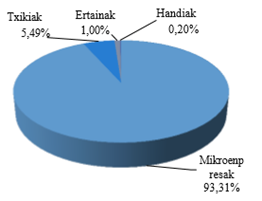
\includegraphics{enpresa_tamaina}
    \centering
    \par{Iturria: \citeauthor{confebask2014dimension} (\citeyear{confebask2014dimension})}
\end{center}

EAEko enpresen tamainari erreferentzia eginez, \ref{fig:enpresa_tamaina} irudian ikus daitekeen moduan, honako hauek dira \citeauthor{confebask2014dimension}-ek (\citeyear{confebask2014dimension}) eskainitako datuak: enpresen \%93,31 mikroenpresak dira eta 10 langile baino gutxiago dituzte; \%5,49 berriz enpresa txikiak dira, hau da, 50 langile baino gutxiago dituzte; \%1 enpresa ertainak dira, gehienez 250 langile dituztenak; eta soilik \%0,2 dira enpresa handiak, 250 langile baino gehiago dituztenak.

Nahiz eta EAEko enpresen kopuru handiena mikroenpresak izan, langileen kopuruaren banaketa enpresaren tamainaren oso bestelakoa da. Hona hemen \citeauthor{confebask2014dimension}ek (\citeyear{confebask2014dimension}) eskainitako datuak, enplegua enpresaren tamainaren arabera:

\begin{center}
    \captionof{figure}{\textit{EAEko langileen banaketa enpresa motako}}
    \label{fig:langile_banaketa}
    \centering
    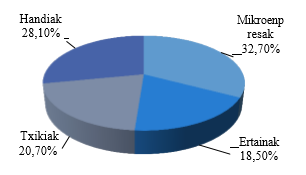
\includegraphics{langile_banaketa}
    \par{Iturria: \citeauthor{confebask2014dimension} (\citeyear{confebask2014dimension})}
\end{center}

\ref{fig:langile_banaketa} irudian ikus daitekeen moduan, mikroenpresek langileen \%32,7 soilik dute, nahiz eta enpresa kopuruaren \%93,31 izan. Enpresa txikien kasuan berriz, langileen \%20,7 enpresa mota hauetan egiten du lan eta ertainetan berriz, langileen \%18,5 aritzen da. Enpresa handien kasuan ordea, nahiz eta enpresa mota hauen kopurua oso murritza izan, langileen \%28,1 ari da bertan lanean.

Enpresa hauen bezeroak munduko herrialde ezberdinetan daude banatuta, enpresetako diru sarrera garrantzitsu bat kanpo merkatuetatik etorriz. Aldi berean, beste herrialde batzuetako produktu ugari ekartzen dira hona egunerokotasunean, esan bezala beste herrialde batzuekiko dependentzia handituz, Covid-19aren testuinguruan argi geratu den moduan. Datuetan sakonduz, \citeauthor{eustat2022kanpo}-en (\citeyear{eustat2022kanpo}) datuen arabera, EAEko ondasunen esportazioak 2619,3 milioi eurokoak izan dira eta inportazioak berriz, 2238,3 milioi eurokoak 2022ko martxoan. Iazko datuekin alderatuz, \%11ko eta \%31ko igoera nominala izan dute, hurrenez hurren.

Aipatutako informazio guztia aztertu ondoren, argi ikusten da aurretik deskribatutako globalizazioaren fenomenoa EAEn ere presente dagoela eta horren parte dela. Azken finean, bertako egoera ekonomiko, politiko, kultural eta soziala erabat baldintzatuta dago mundu mailan dauden joerekiko, nahiz eta tokian tokiko ohitura eta errealitateak pisu handia izan. Teknologia berrien eraginez, distantzia fisikoak desagertu diren heinean, munduko edozein eskualdetan gertatzen denak eragin zuzena eta berehalakoa izan dezake gure eguneroko bizitzan.

Hortaz gain, enpresetako jarduna merkatu berrietara zabaltzeko helburuarekin bertako enpresek nahiz atzerrikoek herrialde ezberdinetan filial eta ofizinak irekitzen dituzte. EAEn ere sektore ezberdinetako multinazional ugarik ireki dituzte egoitzak azkeneko hamarkadetan eta, horrez gain, hainbat proiektu jarri dira martxan instituzioetatik hauekin elkarlanean. Azken finean, globalizazio kontestu batean estrategia garrantzitsuenetako bat enpresen nazioartekotzea da, beren jatorrizko kokapenetatik kanpo dauden merkatuetara bideratzea, ulertuz modu hau dela modu konplexu eta interesgarriena enpresen hazkunde eta garapenerako (\cite{larrinaga2005internacionalizacion}).

Horren adibide dira Amazon, Microsoft eta Google bezalako multinazionalek EAErekiko erakutsi duten interesa eta beraien presentzia bertan handitzeko hartu duten konpromisoa. Amazonen kasuan esaterako Trapagaranen du egoitzetako bat eta Oiartzunen logistikako zentro baten eraikuntzaren proiektua alboratu ondoren, Arabako hainbat lursail aztertzen ari dira hazkunde esponentzialari erantzuteko. Hain zuzen ere, bost aldiz handitu du eta EAEko langile kopurua 2019tik (\cite{irigoyen2021amazon}).

Microsoft enpresa multinazionalaren kasuan berriz, Eusko Jaurlaritzarekin elkarlanean \textit{AI for Earth} proiektuan aritu dira, inteligentzia artifizialean oinarritzen diren proiektu berritzaileak bultzatzeko helburuarekin. Bertatik, bi proiektu jarri dira martxan. Lehena, turbina eoliko flotanteen konportamendua aztertzean datza, energia berriztagarriaren produkzioa maximizatzeko. Besteak berriz, 2018ko udan izan zen onddo defoliatzaileen erasoa hobeto ezagutzea du helburu, etorkizunean gerta daitezkeen egoera berdinei aurre egiteko (\cite{microsoft2020microsoft}).

Adibide hauen bitartez argi ikusten da multinazional hauek duten gaitasun ekonomiko eta zientifikoa arlo oso desberdinetan proiektu ezberdinak martxan jartzeko. Baina aldi berean enpresa hauek estuki baldintzatuta daude hezkuntza esparruan aurrera eramaten diren ikerketa proiektuekin. Horregatik, enpresa handien beharrek hezkuntzaren etorkizuneko norabidea asko baldintzatzen dute, beraien beharrak asebetetzera bidean. Hain zuzen ere, horren adibide garbia da EAEn Euskal Herriko Unibertsitatearen (EHU) \textit{Quantum Center} jarri dela martxan EHUko sei fakultate eta eskoletako 83 ikertzailerekin. Honen helburu nagusia adituak sortzea da enpresen beharrei erantzuteko, eskakizun handia baitago International Business Machines (IBM), Microsoft, Google eta Airbus bezalako multinazionaletatik besteak beste (\cite{gamez2020euskadi}).

\section{GAFAM}\label{sec:gafam}

Multinazional hauen ezaugarritzean sakonduz, sekulako inpaktua dute digitalizazio merkatua kontrolatu eta monopolizatzen duten enpresa teknologiko multinazional nagusiek, eta beraien artean bost erakunde bereizten dira: Google, Apple, Facebook, Amazon eta Microsoft. Bost erakunde hauei erreferentzia egiterakoan GAFAM ezizena erabiltzen da. 

Google, mundu mailan aurki daitekeen bilatzailerik arrakastatsuena da, erabiltzaile gehienek sarean informazio bilaketak egiteko erabiltzen dute orokorrean. Baina, plataforma honen helburuak, lehen puntu honetatik haratago doaz. Bere algoritmoari esker lortu daitekeen ikusgarritasuna kontuan hartuta, plataforma online gehienen muina da. Eskaintzen dituen zerbitzu desberdinak egunetik egunera hazten dira eta hauetako bakoitzak ezaugarri eta funtzionaltasun propioak ditu, erabiltzailearen beharrei modu erakargarri eta berritzaile baten erantzuten dienak.

Amazon, mundu mailan aurkitu daitekeen online denda esanguratsuena da, katalogo guztiz osatu bat eskaintzen diona erabiltzaileari. Kategoria desberdinetan, sektore eta prezio aniztasun handiak kontrolatzen ditu.

Facebook, mundu mailan erabiltzaile gehien konektatzen dituen sare soziala da. Hauen bitartez, pertsonak haien artean konektatzeaz gain, informazioa, eduki audiobisuala, notiziak eta bestelakoak partekatzen dituzte.

Apple, denetariko software eta gailu elektronikoak fabrikatu eta garatzen dituen enpresa multinazionala da. Haien produktu esanguratsuenen artean, \textit{iPod}, \textit{iPhone} eta \textit{iPad}-a daude eta softwareari dagokionez, Applek \textit{MacOS X} sistema operatiboa eta \textit{Safari} web nabigatzaileak garatu ditu.

Microsoft, mundu mailan aurkitu daitekeen software garatzaile garrantzitsuena da. Bere garapen handiena, munduan gehien erabiltzen den \textit{Windows} sistema operatiboa da. Hortaz gain, bere produktu arrakastatsuenen artean \textit{Office suite} ofimatika produktua dago.

GAFAM enpresek, teknologia neutrala eta beti positiboa den ideia transmititzen dute, eta mundua haien arauen arabera interpretatzen dugu. Balore burtsan lehenak dira, azken finean, irakurtzen, entzuten, ikusten dugun guztian interbentzio handia dute: nola lan egiten dugun, nola erosten dugun eta zelan erlazionatu eta dibertitzen garen, besteak beste. Hortaz gain, pandemian zehar hauen erabilera handitu denez, hazkunde mugagabea duten enpresak bihurtu dira (\cite{eavis2020big}).

\textit{Forbes} editorialaren arabera, GAFAM, munduko bost firma baliotsuenak dira. Estatistikak ez daude zuzenki erlazionatuta irabazten duten diruarekin, baina, hauen balioa, diru sarrera gehiago dituen enpresa batenak baino handiagoa da. Azken finean, enpresa mugagabeak, gobernu partiduak, Gobernuz Kanpoko Erakundeak (GKE) eta denetariko elkarteek, enpresa hauek barik bizirautea ezinezkoa da.

\begin{center}
    \captionof{figure}{\textit{GAFAM enpresen etekinen igoera 2019 eta 2020 artean}}
    \label{fig:gafam_etekinak}
    \centering
    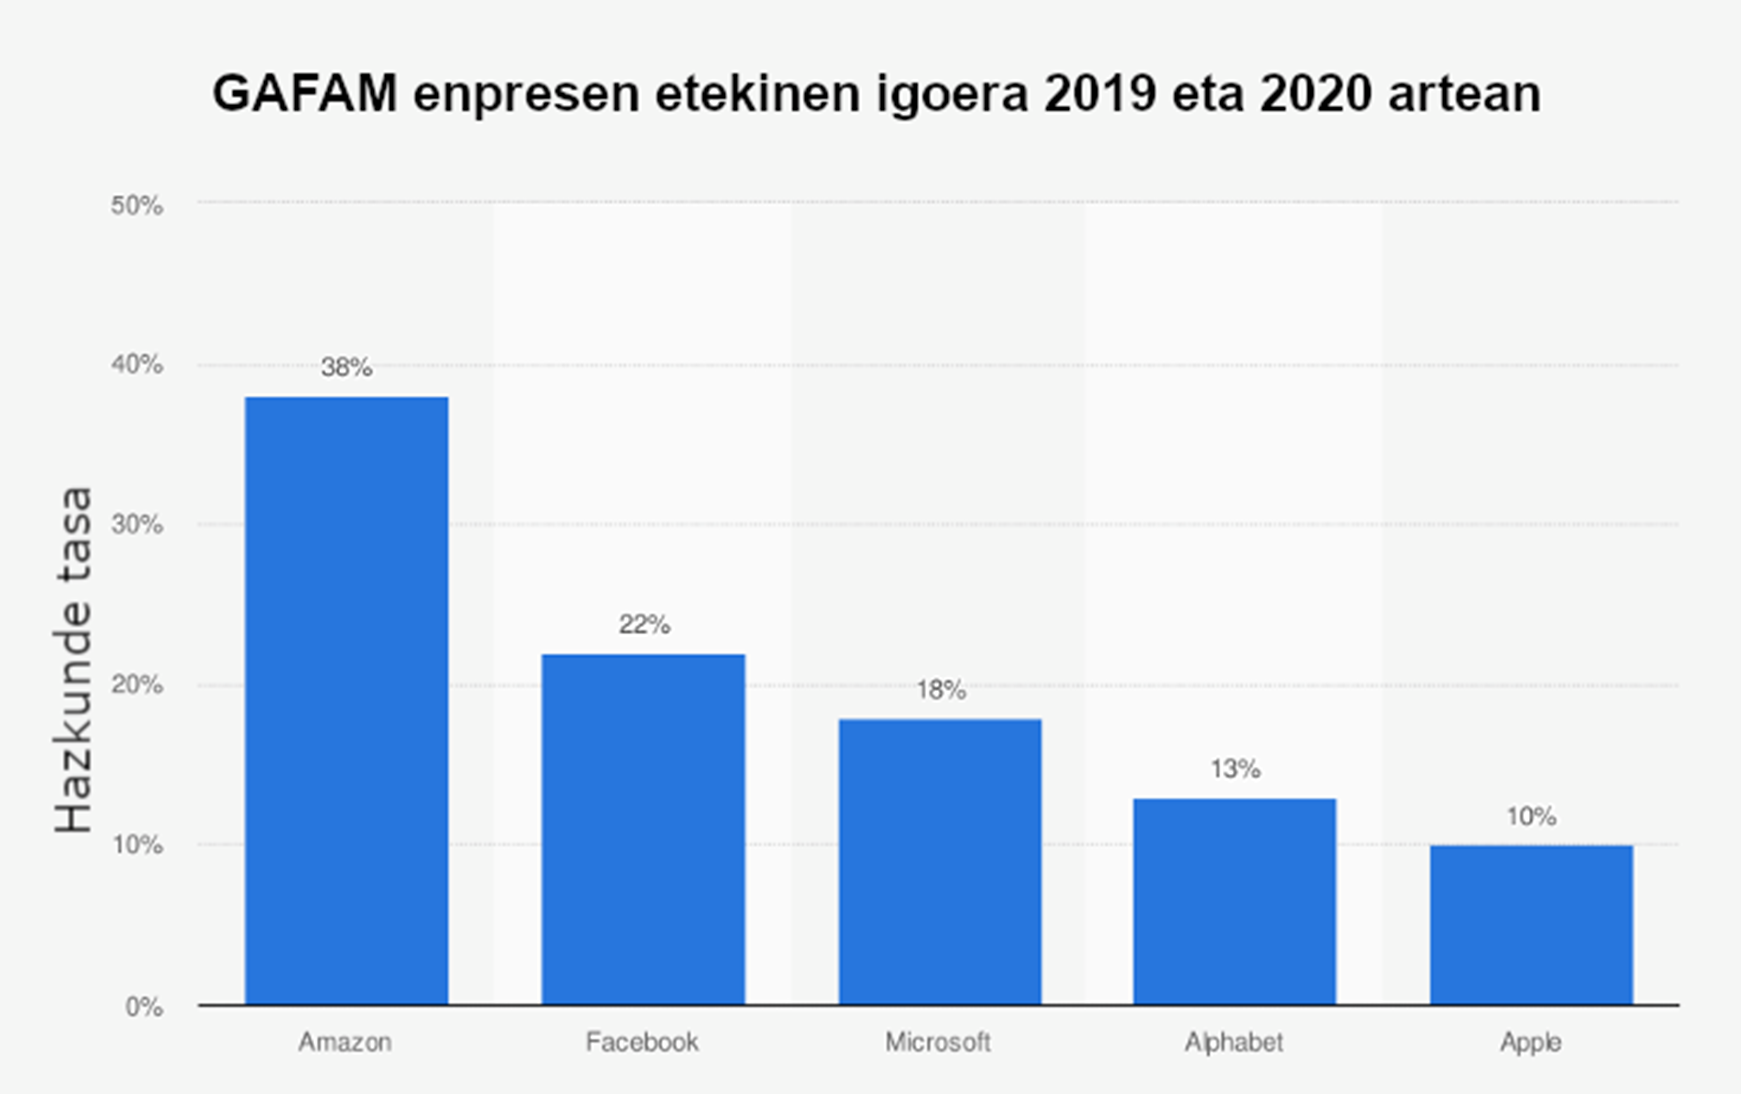
\includegraphics{gafam_etekinak}
    \par{Iturria: Sorkuntza propioa. Abiapuntua: \citeauthor{statista2021gafam} (\citeyear{statista2021gafam})}
\end{center}

Honen eredu argia, 2021 urtean bost enpresa hauek era bateratu batean izan duten irabaziak 259.000 milioi estatubatuar dolar zifra gainditu izana. \ref{fig:gafam_etekinak} irudian ikus daitekeen moduan, 2019 eta 2020 urteen artean GAFAM enpresak izan duten irabazien gorakada nabarmena da.

Monopolio bat mantentzea leporatzen zaie. GAFAM taldea bost enpresa desberdinek osatzen badute ere, ez dira haien arten konpetentzian dauden multinazionalak. Bakoitzak bere esparruan merkatu berriak garatzen lan egiten du eta haien artean sare indartsu eta aberatsa osatzen dute. \citeauthor{thiel2014competition}-ek (\citeyear{thiel2014competition}), PayPal plataformaren fundatzailetako bat, esandakoaren arabera:

\begin{adjustwidth}{3em}{0pt}
"Sare efektuak, produktua geroz eta pertsona gehiagok erabili, produktua erabilgarriagoa bihurtzen dute. Hortaz, erabiltzaile kopurua hain handia izanik, erreza da enpresa hauek sisteman haien arauak inposatzea."
\end{adjustwidth}

Honen inguruan, \citeauthor{de2019guia}-k (\citeyear{de2019guia}) hurrengoa adierazten du:

\begin{adjustwidth}{3em}{0pt}
"Enpresa hauen botereak estatua desafiatzen dute. Bankuen, botere finantzarioak adibidez estatuaren babesa behar duen bitartetan eta haien artean ulertzera behartuta dauden honetan, enpresa teknologikoek botere publikoen gaineko boterea jarduten dute."
\end{adjustwidth}

\section{GAFAM enpresak hezkuntzan zer?}\label{sec:gafam_hezkuntza}

Behin GAFAM enpresak ezaugarrituta, beharrezkoa da hauek hezkuntzaren esparruan eramaten duten jardunaren berri ematea. GAFAM enpresek hainbat helbururekin, nabarmenak edo ezkutukoak izan, haien ekosistema digitalak ikastetxeetan infiltratzeko asmoak argiak dira. Hezkuntzaren industriako erabiltzaileekin konektatu eta haien negozio ereduak, lotura emozionalak edota teknologiara hurbiltzeko forma ezberdinak ezartzea (\cite{herranz2018gafam}).

Hezkuntza mundura hurbildu eta geratzeko etorri dira enpresa hauek. Azken finean, erabiltzailearengan eragina duten ondorengo puntuak erakargarri egiten ditu bere baitan: eskolako bizitza eta bizitza erreala konektatzen dituzte, komunikatzeko eta erlazionatzeko erak aldatuz.

\begin{itemize}
    \item Erabiltzailea ezagutzen dute, izan ere, haien negozio ereduak honetan oinarritzen dituzte.
    \item Erabilera errutina berriak txertatu dituzte, erabiltzailearen esperientzia puntu garrantzitsuenetariko bat da enpresa hauentzat eta ikastetxeek eguneroko bizitzan kontestu desberdinetan hain presente dauden praktikak bereganatu ditu. 
    \item Lan egiteko era berriak, portaera berriak eta orokorrean ohitura aldaketak txertatu dira.
    \item Berrikuntza eta abangoardia hitzak presente daude, hezkuntza Google edo Apple izenekin erlazionatzen diren momentua eta zertifikatu hauek izatea erakargarria egiten dute.
\end{itemize}

Ikuspuntu soziologiko batetatik, generazio berriek positiboki baloratzen dute azkarra eta instantaneoa dena. Hezkuntzak eta ikastetxeak erritmo motelean eta era errepikakor batean aurrera egiten duten bitartean, \citeauthor{herranz2018gafam}ek (\citeyear{herranz2018gafam}), GAFAM enpresek sistema desafiatzen jarraitzen dutela dio proposamen erakargarri eta dinamikoagoekin.

Enpresa hauek, doakotasun faltsua eskaintzen dute ikastetxeetara hurbiltzerako orduan, haien zerbitzuak doan eskainiz, baina estrategia komertzialak besterik ez dira. Benetako asmoa, erabiltzailea ikastetxeko testuinguruan ezagutzea da, horrela hezkuntzaren beharrei erantzuteko negozioa garatzen dute negozio moduan. Hortaz gain, haien ekosisteman bereganatzen zaituzte, hardware, software, erreminta desberdinak, formakuntza eta zertifikatuekin, besteak beste. Honek, beste ekosistemekin konektatzea zailtzen du eta ez da erreza hemendik ateratzea.

Hezkuntza mundura hurbiltzeko asmoak argiak dira, azken finean enpresa hauen hazkunde eta garapenerako erabiltzaile baliotsuak dira. Ondorengo puntuetan enpresa hauen helburuen artean agerikoak direnak aipatzen ditu \citeauthor{herranz2018gafam}ek (\citeyear{herranz2018gafam}): Irabaziak lortzea: hezkuntza sektoreak, fakturazio eta irabazi hazkunde handiak eskaintzen dituen eremua da, aldi berean, negozio linea berriak garatzeko aukera ere.

\begin{itemize}
    \item Irakasle eta ikasleei laguntzea eguneroko lan eta jardueretan.
    \item Erabiltzaile datuak eta datu pertsonalak eskuratzea haien produktuen garapenerako.
    \item Filantropia erabiltzen dute askotan, helburu komertzial oso argiak definituta dituztelarik.
    \item Bezeroak fidelizatzea hauek umeak direnetik. Produktuen bitartez behar berriak sortzen dituzte ikaslearengan, bai eskolako eta bai etxeko esparruetan.
    \item Programazio eta konputazio trebetasunak garatzea ikasleengan, etorkizunean haien langile bihurtu daitezkeen erabiltzailean.
\end{itemize}

Baina, GAFAM enpresek badute hain agerikoak ez diren asmoak eta hezkuntza munduarekin zuzenean kontraesan handiak dituena, \citeauthor{herranz2018gafam}ek (\citeyear{herranz2018gafam}) ondorengo puntuetan deskribatzen dituenak, adibidez:

\begin{itemize}
    \item Enpresa hauek haien estandarrak hezkuntza munduan inposatzen saiatzen ari dira. Irakaskuntzaren praktikan eragina duten formakuntza saioak, doakotasun estrategiak eta zertifikatuak txertatuz.
    \item Hezkuntza zentroetan eta ikaslearen eta irakaslearen bizitzetan algoritmo eta inteligentzia artifizial estrategia masiboak txertatzen dituzte, ikasketa pertsonifikatuaren azken formula izatearen lemarekin.
    \item Datu pertsonalak zertarako erabiltzen dituzten zalantza handia dago oraindik, horien artean: adingabea babesten dute? Zer egiten da haien gailuekin grabatzen den material audiobisual guztiarekin?
\end{itemize}

Filantropiaren ideia faltsua hezkuntzaren bitartez erabiltzen da, non aberatsek eta hauen fundazio "filantropikoak", ez daude donazioen eta laguntzen atzean jada. Aberatsek zuzendu eta bideratzera pasatu dira, non gobernuak, enpresak eta GKEak era bateratu batean lan egiten duten, hezkuntzaren merkatuan dauden hazkunde aukerei heltzeko, politika berriak diseinatuz; edo GAFAM enpresen hedapena "konponbide teknologikoa" eskainiz, hezkuntzaren salbazio eta modernizazio eran apainduta digitalizazioaren bitartez. Baina atzean, XXI. mendeko urrezko negozio ideia dakarrena: etorkizuneko erabiltzaile eta kontsumitzaile generazio oso baten datuak. Hezkuntza eremura adimen artifiziala (\textit{artificial intelligence}, AI), \textit{Big Data}, gauzen interneta (\textit{Internet of Things}, IoT), blokeen katea (edo \textit{blockchain}) edota hodei-konputazioa (\textit{cloud computing}) aplikatuz (\cite{diez2022invasion}).

Posible al da justizia sozialerako bidean lan egiten duten ikastetxeek, software eta hardware produzitzaile multinazionalen instrumentuen erabilera masibo bat egitea? Horregatik, irakasleek, digitalizazio prozesu hauek beraien lanean duten inpaktuaren inguruan pentsatzeko beharra dugu nahitaez. Hausnarketa pedagogiko minimo batek, azalera eramaten du nola plataforma birtual hauek instalatzen duten dinamika berriek gure lan egiteko modua hautatzeko aukerak moztu eta deuseztatzen duten. Hortaz, dialogo aukerak geroz eta txikiagoak diren momentuetan, kritikoa eta elkarrizketarako irekia espiritua nola sortu daitekeen inguruan hausnartu behar da. Edo, lan egiteko eraren kontrola nola berreskuratu behar den, aurretik software diseinatzaileen eskutatik moldeatuta badatoz (\cite{almazan2020covid}).

\section{GAFAM enpresak EAEko hezkuntza sisteman}\label{sec:gafam_eae_hezkuntza}

Laburbilduz, azken hamarkadetan teknologiak eman duen garapen izugarri baten kontestuan eta digitalizazio prozesu etengabe batean aurkitzen da gizartea. Honek guztiak, erabiltzailearentzat bere datuen gaineko kontrolaren erabateko galera suposatu du. Aldi berean, enpresa handi gutxi batzuen esku geratuz informazio guztia, irabaziak lortzeko bitarteko bihurtuz (\cite{decode2017what}). Egoera honetan, datu kantitate horiek ez dira erabilgarriak onura publikorako zerbitzu eta irtenbideak sortzeko. Kontrara, honek desberdintasun ekonomikoak eta eraginkortasun eza ekartzen ditu.

EAEren kasuan ere, ikus daiteke hezkuntzaren digitalizazioaren bidean Eusko Jaurlaritzak hartu duen norabidea eta aldi berean, horri aurre egiten dioten proposamenen garapena. 2022eko apirilean, Eusko Jaurlaritzak Google, teknologia digitalen enpresa multinazional pribatuaren tresnak ikastetxe publikoetan erabiltzeko, gutxienez lau urterako hitzarmena sinatu zuen. Hezkuntza Saileko ikastetxeetan \textit{Google Workspace for Education} zerbitzuak erabiltzeko hitzarmena sinatzen dute \textit{Google Cloud Emea Limtied} enpresak eta Eusko Jaurlaritzak eta bi aldeek hainbat konpromiso hartu dituzte. Horrela dio \citeauthor{apaolaza2022google}-k (\citeyear{apaolaza2022google}):

\begin{adjustwidth}{3em}{0pt}
“Hezkuntza Sailak Googlen zerbitzuak ezartzeko faseak definituko ditu eta zerbitzu horietarako sarbideak erraztuko dizkie irakasle zein ikasleei, baita beharrezko “prestakuntza-planak” egin ere. Gainera, Googlekin “lankidetzan” aritzeko konpromisoa hartu du Hezkuntza Sailak; talde misto bat sortuko dute horretarako, eta “tresna berriak probatzeko” \textit{betatester} talde bat ere sortuko dute ikasleen artean, ikastetxeetan Googlen zerbitzuen erabilera sustatzeaz gain.”
\end{adjustwidth}

\citeauthor{ej2022aldizkari}-ren (\citeyear{ej2022aldizkari}) aldizkariak jasotzen duen hitzarmenak, bai Eusko Jaurlaritzak eta bai Googlek sinatutako baldintzak irakurri daitezke. \citeauthor{apaolaza2022google}ren (\citeyear{apaolaza2022google}) hitzetan oinarrituz, aldizkariak arrazoi ekonomikoak ez ditu inondik inora azaltzen. Gainera, Google enpresa bat izanez, etekina aterako duela jakina da, baina hau ere ez da adierazten. Gazteen erabilerarekin lortutako datu pertsonalen tratamendua eta erabileran oinarrituko dela ondorioztatu daiteke. Erabaki honen bitartez, Eusko Jaurlaritzak Hezkuntza Sailaren menpeko ikastetxeetako ikasleen datuak pribatizatzearen alde egin du.

Googlerekin sinatutako azken hitzarmen honetaz gain, Eusko Jaurlaritzak harreman historikoa du Microsoftekin eta eskoletako digitalizazioa enpresa honen esku utzi du. \citeauthor{barcenilla2021gv}-k (\citeyear{barcenilla2021gv}) jasotzen duen moduan, “EAEko eskola publikoetan ikasleek erabiltzen dituzten plataforma digitalak Microsoftekin hitzartu ditu Eusko Jaurlaritzak, bost urtean multinazionalera 3 milioi euro bideratuz”. Sare publikoa osatzen duten EAEko ikasleen \%51 Microsoften datu-basean daude. 

Enpresa multinazional hauek hezkuntza sistemaren barruan daude jada eta Google eta Microsoft enpresek sortutako erremintak eta aplikazioak Euskal Herriko ikastetxe pribatu eta publiko ia guztietan erabiltzen dira.

Erabaki honen aurrean kritiko diren norbanako eta eragileak azaltzen dute software itxi hauek, hezkuntza sistemaren barruan sarbidea izateak, ikasle adingabeen datuak eta hauen eskubide urraketan eragin larria duela. Doakotasun faltsua eskaintzen dute eta trukean datu pertsonalak eskuratzen dituzte. \citeauthor{hl2019komunikatua} \citeyear{hl2019komunikatua} taldearen ustez, enpresa pribatuek egin dute digitalizazioaren gidaritza orain arte, eta planik ez dago Eusko Jaurlaritzako Hezkuntza Sailean. Horrela bada, hezkuntza eredu burujabeago batera bultzatzeko nahian mugimendu ezberdinak sortu behar dira, zentroetan software libreak inplementatuz, adibidez.

\section{Burujabetza digitala eta hezkuntza librezalea}\label{sec:burdig}

Kontestu honetan egitasmo ezberdinak sortu dira aipatutako egoera honi buelta eman asmoz, erronka digitala XXI. mendeko erronka nagusi moduan hartuz. Aipatzekoa da \citeauthor{ehd2021manifestua}k (\citeyear{ehd2021manifestua}) argitaratutako manifestua, teknologia jendartearen zerbitzura jartzeko helburuarekin. Hauen esanetan, auzi honek 4 esparrutan eragin du gutxienez: Demokraziaren esparruan, lanean, hezkuntzan era gizakian berarengan. 

Hezkuntzaren esparruan duen eraginak kezkatuta, Euskal Herrian alternatibak planteatzera bidean, 2017an Hezkuntzan ere Librezale taldea jarri zen martxan, irakasle, ikasle, guraso eta eragileez osatua. Hainbat puntuz osatutako komunikatu bat dute kaleratua eta zenbait material eskuragarri dute euskal hezkuntzan ematen den egoeraren aurrean alternatiba digital libreen erabilera bultzatzeko (\cite{hl2019komunikatua}). Hainbat kezka mahaigaineratzen dituzte:

\begin{itemize}
    \item Ikasleen datuak enpresa pribatuen esku uzteak beraien pribatutasuna galarazten du, ikaslea produktu bihurtuz. 
    \item Chromebook bezalako gailuetan inbertsioak egitea arduragabekeria da, 5 urteren buruan zaharkituak geratzen direlako, berrerabilpena galaraziz.
    \item Gailu digitaletan euskararen presentzia enpresa pribatuen agindu eta nahietara uztea euskararen aurkako neurria da. Konkretuki, Chromebooketako hainbat atal ez daude euskaraz gaur egun. 
    \item Ikasleei tresna digital berdinak erabiltzera mugatzea, hezkuntza digitala murriztea da.
    \item Hezkuntza komunitatean tresna hauekiko dependentzia sortzea arazo larria da. Instituzioetatik enpresa pribatuen erabiltzaile eta bezeroak sortzen ari dira. 
\end{itemize}

Honen aurrean, ikasleen eskubide digitalak eta pribatutasuna errespetatuz eta bitarteko teknologiko auditagarri, berrerabilgarri, libre eta gardenak erabiliz, digitalizazio etiko, arduratsu, eraginkor eta euskalduna bermatzeko aukerak sortu behar dira (\cite{hl2019komunikatua}). 

Hori epe luzerako begiradarekin diseinatu behar da gure hezkuntza sistema bere burua eraldatzen joan dadin, baita digitalizazioan ere. Digitalizazioak hezkuntzari aukera askotarikoak eskaintzen dizkio, beti ere, ikaslearen ahalduntzearekin zuzenean lotuak. Ahalduntze horrek, gaitasun digitalak garatzeaz haratago, menpekotasunak sortzea saihestu eta ikasleak ingurune digitalean boterea hartzea eskatzen du, herritar digital burujabeak izan daitezen (\cite{hl2019komunikatua}).

Bide honetan, ikastetxeko datuak multinazional handien esku uzteari aurre eginez, software libreen erabileraren alde pausuak eman dituzte hainbat ikastetxetan. Tolosako Lanbide Heziketako zentroan 3 produktu nagusi dituzte martxan: Postarako \textit{Zimbra}, klaseak kudeatzeko \textit{Moodle} eta \textit{NextCloud} informazioa artxibatzeko hodei moduan (\cite{garcia2020}). Beste adibideetako berriz, Elgoibarko Fabrikazio Aurreratuaren era Digitalaren Campusa izango litzateke. 

Euskal Herrian eman diren adibide hauez gain, estatuko beste hainbat lekutan, nahiz, Europa mailan hainbat egitasmo jarri dira martxan. Esaterako, Katalunian \textit{Xnet} eskubide digitalen plataformak aurkeztu duen \textit{Digital Democràtic} suitea. Honek, ikastetxe eta hezkuntza esparruari erreminta digital ugari eskaintzen dizkie, software libre eta auditagarria bat esaterako. Honen asmoa Google \textit{Meets}, \textit{Drive} edo \textit{Calendar} bezalako tresnak ordezkatzea. Plataforma hau, Google bezalako multinazionalen aurrean alternatibarik ez zegoelako jaiotzen da 2018 urtean (\cite{vicente2022}). Horrez gain, Valentziako erkidegoa da ikasleen pribatutasuna babesteko kode irekiko tresnak diseinatu dituen Europar Batasuneko eskualde bakarra (\cite{barcenilla2021gv}).

Bukatzeko, beste adibideetako bat \citeauthor{decode2017what} \citeyear{decode2017what} proiektu esperimentala da, zeinak, helburu moduan alternatiba praktikoak sortzea duen, pertsonen datuak babestu eta burujabetza digitala bultzatzeko. Hau Europa mailan landutako saiakera da. 